\documentclass[runningheads]{llncs}

\usepackage[T1]{fontenc}
\usepackage{graphicx}
\graphicspath{ {figures/} }
\usepackage{array}
\usepackage{hyperref} 
\usepackage{amsmath}
\usepackage{mathabx}
\usepackage{multirow}
\usepackage[printonlyused,withpage]{acronym}
\usepackage{algorithm}
\usepackage{algorithmic}
\usepackage{listings}
\usepackage{xcolor}

\setcounter{tocdepth}{3}

\makeatletter
\renewcommand\maketitle{
  \begin{center}
    {\LARGE\bfseries \@title \par}
    \vskip 1em
    {\small\lineskip .5em%
     \begin{tabular}[t]{c}\@author
     \end{tabular}\par}
    \vskip 1em
    {\footnotesize\@institute\par}
  \end{center}%
}
\makeatother


\begin{document}

\title{Satisfiability Problem with MiniSat - Benchmarks, Comprehension and Challenges}

\author{Șova Dumitru Ștefan Andrei, \email{dumitru.sova01@e-uvt.ro} 
\and Andries Rafael Gabriel, \email{rafael.andries00@e-uvt.ro} 
\and Stoentel Alexandru-Eduard, \email{alexandru.stoentel01@e-uvt.ro} 
\and Nenescu Eugeniu \email{eugeniu.nenescu00@e-uvt.ro}}

\authorrunning{F. Author et al.}

\institute{West University of Timișoara, Bulevardul Vasile Pârvan 4, Timișoara 300223}

\addtocontents{toc}{\protect\setcounter{tocdepth}{0}}

\maketitle 
\addtocontents{toc}{\protect\setcounter{tocdepth}{3}}

\begin{abstract}

For as long as we have been alive, logic has helped us make sense of the world surrounding us, from our philosophical inquiries to its use in modern mathematics and informatics. Logic bridges the gap between formal and informal knowledge, proving essential in databases, programming languages (\ac{e.g}, Prolog), and propositional logic. This paper focuses on a compelling area within informatics: the \ac{SAT}. Our main focus will be on MiniSat, a \ac{SAT} solver designed to efficiently address the challenge of satisfiability. Such solvers can tackle problems with millions of variables, benefiting research and industry.

This report will include the installation process for MiniSat, initial challenges faced with working with MiniSat, benchmarks from recent \ac{SAT} competitions, mainly the Hamiltonian family of tests, a look into the algorithms found in the code of MiniSat, and suggestions on how the code might be modified to improve runtimes. Our analysis will highlight MiniSat’s capabilities, while the code and benchmarks can be found in the following GitHub link: 

\url{https://github.com/AndiSova/VF-Software-Engineering-2024-Project}

\keywords{MiniSat  \and \ac{SAT} \and algorithms.}
\end{abstract}

\lstset{
    frame=none,
    language=C++,
    numbers=none,
    tabsize=4,
    showstringspaces=false,
    basicstyle=\ttfamily,
    keywordstyle=\color{violet},
    commentstyle=\color{green},
    morekeywords={Vec, Constr, Solver, NULL, true, false}
}

\newpage
\tableofcontents
\listoftables
%\listoffigures
{\noindent \large \textbf{List of acronyms}\par}

\begin{acronym}
 \acro{SAT}{Boolean satisfiability problem}
 \acro{e.g.}{example}
 \acro{NP-complete}{Nondeterministic Polynomial-Time complete}
 \acro{EDA}{electronic design automation}
 \acro{DPLL}{Davis Putnam Logemann Loveland}
 \acro{CDCL}{Conflict-Driven Clause Learning}
 \acro{UML}{Unified Modeling Language}
 \acro{CNF}{Conjunctive Normal Form}
 \acro{WSL}{Windows Subsystem for Linux}
 \acro{OS}{Operating System}
\end{acronym}
\newpage

\section{Introduction}\label{cap:intro}

\ac{SAT} is a cornerstone in computational theory and practical applications, namely \ac{EDA}, artificial intelligence, and combinatorial optimization (see \cite{sat-solver}). Since 2003, MiniSat has continued to be a small, efficient, and readable \ac{SAT} solver, representing a perfect tool to introduce students and professionals alike to the nuances of \ac{SAT} solving (see \cite{minisat}).

While MiniSat is often praised for its straightforward design, working with it as a beginner can present various challenges. For example, setting up MiniSat, understanding its algorithms, such as \ac{DPLL} and \ac{CDCL}, and running your first benchmark might challenge the uninitiated.

In this report, we will explore these challenges from the perspective of newly introduced users. Our study includes the steps for installing MiniSat, the steps required to run a test from the 2024 \ac{SAT} competition, an analysis of MiniSats' main algorithms, possible improvements that can be made for the source code, and the results from running a family of tests using the original code. 

For a better understanding of the main components of MiniSat, we will apply principles from software engineering, making use of \ac{UML} diagrams and detailing the code, using pseudocode, in an attempt to bridge the gap between theoretical concepts and practical implementation.

\subsection{Motivation}\label{sect:Motivation}

Our main motivation for studying MiniSat stems from its influential role in advancing \ac{SAT} solver technology and its accessibility as a learning tool. Since 2003, MiniSat has set a standard for efficiency in solving \ac{SAT} problems, providing a straightforward and readable code that allows us to delve into its algorithms and structure. 

It represents a perfect starting line for our introduction into the world of \ac{SAT} solvers and their particularities, showcasing powerful algorithms, such as \ac{DPLL} and \ac{CDCL}, while also allowing us to explore potential improvements for the current code.

\subsection{Scope and Objectives}\label{sect:Scope and Objectives}

With its ease of use in mind, without prior knowledge, the use and understanding of MiniSat might seem harder than it is. As such, our main aim for this paper will be to showcase how one can use MiniSat, as a first-time user, how to run a benchmark for the first time, how to understand the code that MiniSat runs on, and to start a discussion on how the code could be improved in the future.

\newpage

\section{SAT problem and solutions}\label{cap:SAT problem and solutions}
\subsection{Problem description}\label{sect:Problem Description}

The \ac{SAT} problem in propositional logic asks to determine in a given formula that combines atomic propositions using the Boolean operators "and" ($\land$), "or" ($\lor$), and "not" ($\neg$), whether there are truth values for the atoms in the formula such that the formula evaluates to true\cite{SAT}. In summary, the \ac{SAT} problem is the challenge of determining if a logical formula, typically represented in \ac{CNF}, has at least one solution.

While it is possible to be resolved by hand, after a certain number of atoms, the solution for such formulas becomes increasingly harder to be determined by ourselves alone, resulting in the need for solvers similar to MiniSat to exist. This exponential increase in difficulty for solving complex formulas has fueled the development of \ac{SAT} solvers, which apply advanced algorithms to handle these formulas efficiently.

With \ac{SAT} solvers like MiniSat, designed specifically to tackle these computational hurdles, we reached a level where it is possible to solve these problems within a reasonable time slot.

\subsection{MiniSat installation and first challenges}\label{cap:MiniSat installation and first challenges}

Since the installation process for MiniSat on the Windows \ac{OS} is not the most straightforward, this paper will showcase how a new user can install the solver on their machine with the following instructions:

To begin using the solver, we will go for the \ac{WSL} approach, which allows us to run a Linux environment natively on Windows without the need for virtual machines or terminals such as Cygwin. Below are the steps followed for the installation process:

Firstly, \ac{WSL} needs to be enabled, to do this, the following command is required to be run in PowerShell(mandatory, Powershell needs to be run as an Administrator):
\begin{verbatim}wsl --install\end{verbatim}

This command installs the required features and the default Linux distribution (Ubuntu) system for \ac{WSL}. However, in some cases, users may encounter issues where the installation hangs or doesn't complete. To resolve this, it's necessary to ensure that Windows is fully updated and that the proper components for \ac{WSL} 1(or version 2 if the user chooses so) are manually enabled. This can be done again in PowerShell(running in Administrator mode) using the following commands: 
\begin{verbatim}dism.exe\end{verbatim} 
This command was used to enable Virtual Machine Platform features. After successfully running it, the following command needs to be run to ensure \ac{WSL} 1 is set as the default version.
\begin{verbatim}wsl --set-default-version 1 \end{verbatim}  

In the possibility that neither command works, another possible solution would be to manually install the following update for Windows, wsl$\_$update$\_$x64, which allows Linux environments to run directly on Windows.

After enabling \ac{WSL}, we need to install Ubuntu, a Linux-based \ac{OS}. To do this, Ubuntu can be installed from the Microsoft Store or its home site(for this paper, version 22.04 of Ubuntu was chosen). To complete the installation process, a username and password need to be set up by the user. It is highly recommended to update Ubuntu after we are done with the setup process. We will use the following command to do so: \begin{verbatim}sudo apt update\end{verbatim}

Installing MiniSat on Ubuntu: First, we will install the MiniSat solver by running: \begin{verbatim}sudo apt install minisat\end{verbatim}

\subsection{First benchmark}\label{First benchmark}
With MiniSat successfully installed, we can run the solver and evaluate its performance. To ensure that MiniSat is working properly, we can first test its basic functionality by running a sample input. To do this, we need to open the Ubuntu terminal and type the following command: \begin{verbatim}minisat\end{verbatim} This should display MiniSat’s usage instructions, confirming that the installation was indeed successful.

Next, to run a benchmark, we use test instances from recent SAT competitions. These competitions provide SAT instances that can be used to evaluate the efficiency and performance of various solvers, including MiniSat.

To run a benchmark, we can follow these steps:

- We will use the following link to download our tests: 

\url{https://benchmark-database.de/?track=main_2024}. 

- On the first page, we see several rows, each with a hash code on them. We need to select one of the hash codes to download the file in .cnf format.

- If we wish to search a specific family of tests, on the top of the page there is a 'Query for instances' search bar. Here, we can write a query to receive only the tests we are interested in. For example, if we wish to fetch only the tests from the 2024 competition of the Hamiltonian family, we need to run: 
\begin{verbatim}track=main_2024 and family like Hamiltonian\end{verbatim}

- After choosing which test we wish to download, we need to click on the hash code from the test and a download process will start. The file downloaded is a .zip file, which we need to unzip, in it we can find the .cnf file that we need.

- Having downloaded the test file, we need to place it inside our Ubuntu folder first. To find it, in File Explorer, in the file search bar, we can type \begin{verbatim}\\wsl.localhost\Ubuntu-22.04\home\username\end{verbatim} to easily access it. 

- After placing the file in the correct folder, we can use the following command to have MiniSat try and solve it: 
\begin{verbatim}minisat <benchmark_file>.cnf output.stats > output.out\end{verbatim}

This command will create 2 files in the folder where we placed our test file, a .stats file where we can see the total runtime, whether the formula is satisfiable or unsatisfiable, and the memory used, and a .out file where the results are shown, showcasing as well which literals are true and which are false.

As seen, some challenges might arise from installing MiniSat, as such, we looked into installing MiniSat using different means, for example by using Cygwin, and by installing it using a Virtual Machine. However, we observed that installing it using \ac{WSL} can prevent certain problems. Virtual Machines do not use the system's full power, which is desirable when running benchmarks. Cygwin provides a harder and more complex installation process than PowerShell and Ubuntu.

\section{Code Documentation}\label{cap:Code Documentation}

To better understand the MiniSat solver, we will delve into some of its most important algorithms, namely, the \ac{CDCL} and \ac{DPLL} algorithms. We will also look in this section at possible ways in which we could improve the current code in the future.

The following diagram showcases the main use cases of MiniSats' code:

\begin{figure}
    \centering
    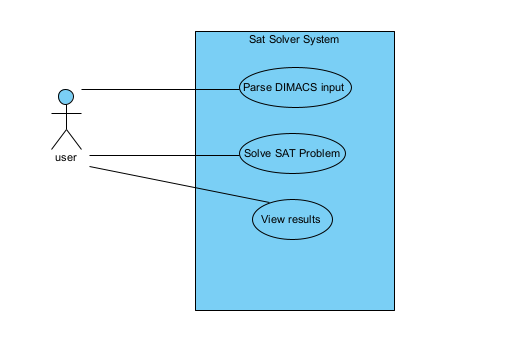
\includegraphics[width=0.67\linewidth]{usecase.png}
    \caption{Use Case Diagram}
    \label{fig: Use Case Diagram}
\end{figure}

\subsection{Algorithm structures}\label{Algorithm structures}

The \ac{DPLL} algorithm is a method used to solve Boolean satisfiability problems (SAT). In simpler terms, it’s a systematic way to figure out whether there’s a way to assign true or false values to a set of variables so that a logical formula becomes true \cite{DPLL}.

The \ac{CDCL} algorithm is an advanced method used to solve Boolean satisfiability problems (SAT). It builds on the basic ideas of the \ac{DPLL} algorithm but introduces several powerful techniques to solve problems faster and handle more complex cases \cite{CDCL}.

Now we'll go by each file in the MiniSat code and see where and how these 2 algorithms are used. The code can be found on the project GitHub link, here: \url{https://github.com/AndiSova/VF-Software-Engineering-2024-Project/tree/main/minisat}

In the main.cc file, in the core folder, both algorithms are used, we'll first talk about the \ac{CDCL} algorithm. The Solver class serves as the primary implementation of the algorithm while the solverLimited() method is the core of it handling tasks like conflict analysis, decision making, and propagation.
The Lit data structure is utilized to represent Boolean variables and their negations while the interrupt() method allows the solver to be halted a common feature in \ac{CDCL} solvers.

Now we'll move on to the \ac{DPLL} algorithm in the same file.
The simplify() method carries out unit propagation and pure literal elimination, both fundamental components of the \ac{DPLL} algorithm.
DIMACS format parsing is implemented, allowing the solver to handle the standard input format commonly used by \ac{SAT} solvers based on \ac{DPLL}.

The responsibilities of the main function are as follows :

- Parses command-line arguments and configures the solver appropriately.

- Reads and processes the input DIMACS file (from a file or standard input) using the parse$\_$DIMACS() function.

- Executes the simplify() method for unit propagation and pure literal elimination.

- Calls the solveLimited() method to solve the \ac{SAT} problem using the \ac{CDCL} algorithm.

- Outputs the result (SAT, UNSAT, or indeterminate) and, if specified, writes the solution to an output file.

Now we're gonna move on to the Solver.cc file in which we find the main components of the \ac{CDCL} solver which are as follows :

- Propagation: The propagate() function performs unit propagation, identifying and enqueues implied literals based on the current assignment\cite{sat-solver}. The following pseudocode\cite{sat-solver} showcases how propagate() works:

\begin{lstlisting}
Constr Solver.propagate()
    while (propQ.size() > 0)
        // `p' is now the enqueued fact to propagate
        lit p = propQ.dequeue();
        // `tmp' will contain the watcher list for 'p'
        Vec(Constr) tmp;       
        watches[index(p)].moveTo(tmp);

        for (int i = 0; i < tmp.size(); i++)
            if (!tmp[i].propagate(this, p))
                // Constraint is conflicting
                // copy remaining watches to 'watches[p]'
                // and return constraint:
                for (int j = i+1; j < tmp.size(); j++)
                    watches[index(p)].push(tmp[j]);
                propQ.clear();
                return tmp[i];
    return NULL;
\end{lstlisting}

- Conflict Analysis: The analyze() function analyzes a conflict clause to decide the asserting literal and appropriate backtrack level so that we can resolve the conflict\cite{sat-solver}. The following pseudocode\cite{sat-solver} showcases how analyze() works:

\begin{lstlisting}
void Solver.analyze(Constr confl, // 
                Vec(lit) out_learnt, Int& out_btlevel)
    Vec(bool) seen(nVars(), FALSE)
    int counter = 0
    lit p = ~lit
    Vec(lit) p_reason
    // Leave room for the asserting literal
    out_learnt.push()  
    out_btlevel = 0
    do
        p_reason.clear()
        // invariant here: confl != NULL
        confl.calcReason(this, p, p_reason)  
        // Trace reason for p:
        for (int j = 0; j < p_reason.size(); j++) 
            lit q = p_reason[j]
            if (!seen[var(q)]) {
                seen[var(q)] = TRUE
                if (level[var(q)] == decisionLevel())
                    counter++
                // exclude variables from decision level 0
                else if (level[var(q)] > 0)  
                    out_learnt.push(~q)
                    out_btlevel = max(out_btlevel, level[var(q)])
        // Select the next literal to look at:
        do
            p = trail.last()
            confl = reason[var(p)]
            undoOne()
        while (!seen[var(p)])
        counter--
    while (counter > 0)
    out_learnt[0] = ~p
\end{lstlisting}

- Clause Database Management: The solver includes functions to manage the clause database effectively such as reduceDB() which periodically removes less active learned clauses to maintain efficiency and removeSatisfied() which eliminates clauses that are already satisfied\cite{sat-solver}. The following pseudocode\cite{sat-solver} showcases how reduceDB() works:

\begin{lstlisting}
void Solver.reduceDB()
    int i, j
    double lim = cla_inc / learnts.size()
    sortOnActivity(learnts)
    for (i = j = 0; i < learnts.size() / 2; i++)
        if (!learnts[i].locked(this))
            learnts[i].remove(this)
        else
            learnts[j++] = learnts[i]
    for (; i < learnts.size(); i++) 
        if (!learnts[i].locked(this) && learnts[i].activity() < lim)
            learnts[i].remove(this)
        else
            learnts[j++] = learnts[i]
    learnts.shrink(i - j)
\end{lstlisting}

- Decision Heuristic: The pickBranchLit() function selects the next decision variable and its polarity based on variable activity, helping guide the search process.

- Restarts: The search() function incorporates a restart strategy, assuming and propagating until a conflict is found, with support for using the Luby sequence to determine restart intervals, improving solver performance on challenging problems\cite{sat-solver}. The following pseudocode\cite{sat-solver} showcases how search() works:

\begin{lstlisting}
bool Solver.search(int nof_conflicts, //
            int nof_learnts, SearchParams params)
    int conflictC = 0
    var_decay = 1 / params.var_decay
    cla_decay = 1 / params.cla_decay
    model.clear()

    loop
        Constr confl = propagate()
        if (confl != NULL)
            // Conflict
            conflictC++
            Vec(lit) learnt_clause
            int backtrack_level
            if (decisionLevel() == root_level)
                return FALSE
            analyze(confl, learnt_clause, backtrack_level)
            cancelUntil(max(backtrack_level, root_level))
            record(learnt_clause)
            decayActivities()
        else
            // No conflict
            if (decisionLevel() == 0)
                // Simplify the set of problem clauses:
                // our simplifier cannot return false here
                simplifyDB()
            if (learnts.size() / nAssigns() >= nof_learnts)
                // Reduce the set of learned clauses:
                reduceDB()
            if (nAssigns() == nVars())
                // Model found:
                model.growTo(nVars())
                for (int i = 0; i < nVars(); i++)
                    model[i] = (value(i) == TRUE)
                cancelUntil(root_level)
                return TRUE
            else if (conflictC >= nof_conflicts)
                // Reached bound on the number of conflicts:
                // force a restart
                cancelUntil(root_level)
                return FALSE
            else
                // New variable decision:
                // may have a heuristic for polarity here
                lit p = lit(order.select()) 
                // cannot return false
                assert(decisionLevel() > 0) 
\end{lstlisting}

- Garbage Collection: The garbageCollect() function reclaims unused memory by relocating clauses and reasons to a new memory region, ensuring efficient memory usage.

Next is the Dimacs.h file.
The \ac{DPLL} implementation in the Dimacs.h file focuses on handling the DIMACS input format, which is widely used by \ac{SAT} solvers. 

This file contains key functions for parsing and processing the input to prepare it for solving:

- readClause() Function: This function reads individual clauses from the DIMACS input and adds them to the solver's internal database. It's a critical step in setting up the problem for the DPLL algorithm.

- parse$\_$DIMACS$\_$main() Function: This is the main parser loop that processes the DIMACS file. It reads the header and clauses, ensuring they are correctly added to the solver. This function plays a central role in initializing the DPLL algorithm.

- parse$\_$DIMACS() Function: A wrapper around the main parser, this function handles the setup of the input stream and calls the core parsing logic.

The last but not least is the Solver.h file.
The Solver.h file contains the core methods and structures for implementing both the \ac{CDCL} and \ac{DPLL} algorithms, as well as essential supporting components:

\ac{CDCL} Algorithm:

- The solve() and solveLimited() Methods: These are the main entry points for solving SAT problems using the CDCL approach.

- The analyze() Method: Performs conflict analysis and clause learning, which are key features of CDCL, enabling the solver to avoid repeating mistakes.

- The propagate() Method: Handles unit propagation and detects conflicts during the solving process.

- Decision Levels and Search State Tracking: Utilizes decision levels, reasons for variable assignments, and a trail to manage and monitor the current state of the search.

\ac{DPLL} Algorithm:

-The simplify() Method: Executes unit propagation and pure literal elimination, the foundational steps of the DPLL algorithm.

-The enqueue() Method: Assigns values to variables during the solving process, helping to progress the search. The following pseudocode\cite{sat-solver} showcases how enqueue() works:

\begin{lstlisting}
bool Solver.enqueue(lit p, Constr from = NULL)
    if (value(p) != l)
        if (value(p) == FALSEL)
            // Conflicting enqueued assignment
            return false;
        else
            // Existing consistent assignment 
            // - don't enqueue
            return true;
    else
        // New fact, store it
        assigns[var(p)] = lbool(!sign(p));
        level[var(p)] = decisionLevel();
        reason[var(p)] = from;
        trail.push(p);
        propQ.insert(p);
        return true;
\end{lstlisting}

Supporting Components:

- Watcher Lists and watches Data Structure: Efficiently monitors watched literals to optimize propagation.

- order$\_$heap Priority Queue: Maintains an ordering of decision variables based on variable activity, improving the efficiency of the decision heuristic.

- Clause Management: Includes operations for attaching, detaching, and removing clauses as needed.

- Variable Activity Maintenance: Tracks and adjusts variable activity with a decay mechanism, ensuring the decision heuristic remains effective.

The combination of these methods and components in Solver.h and all the other files analyzed provide the foundation for robust SAT solving using both the \ac{CDCL} and \ac{DPLL} algorithms.

The following diagram showcases the relations between the classes that we talked about:

\begin{figure}
    \centering
    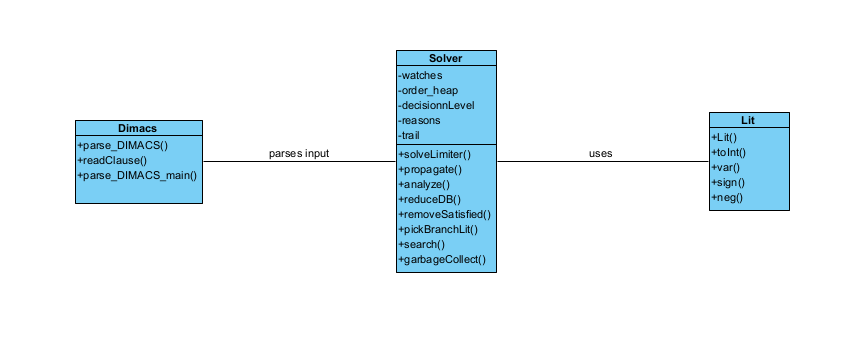
\includegraphics[width=1\linewidth]{classdiagram.png}
    \caption{Class Diagram}
    \label{fig: Class Diagram}
\end{figure}

\subsection{Future Improvements}\label{Future Improvements}

Our proposed improvement to the MiniSat code revolves around the Clause Deletion policies.

MiniSat currently decides which learned clauses to keep by tracking how often they're involved in conflicts. Each clause gets a score that goes up when it helps find conflicts and slowly decreases over time. While this works okay, it has a problem - it often throws away clauses that are good at simplifying the formula just because they don't cause many conflicts.

The strategy that we want to implement makes MiniSat smarter about which learned clauses to keep. Instead of just counting how many conflicts a clause causes, it looks at how often the clause helps simplify the problem through unit propagation. This means keeping useful clauses that guide the solver in the right direction, even if they don't directly cause conflicts. The deletion rules also adapt based on solver performance, which helps maintain efficiency.

By doing this, we want to improve how we delete clauses by looking at how often they help with propagation, not just conflicts. This way, we keep clauses that are good at simplifying the problem, even if they don't cause many conflicts, thus achieving a better balance of memory use and performance, which should help solve complex problems faster.


\newpage

\section{Experimental Results}\label{Experimental Results}

The following experimental results for the Hamiltonian family of tests were taken from the following link: \url{https://benchmark-database.de/?track=main_2024}. For the test, the following computer with the mentioned specs was used: 
OS: Windows 11 Pro,
Processor: 12th Gen Intel(R) Core(TM) i5-12500H 2.50 GHz,
RAM: 16,0 GB (15,8 GB usable).

\renewcommand{\arraystretch}{0.8}
\begin{table}[h!]
  \centering
  \begin{tabular}{|c|c|c|c|}
    \hline
    \cline{2-4}
    hash & SAT/UNSAT & Memory used (MB) & Runtime (s) \\
    \hline
    3a75ad246dbc750a7391ad887c5b0835 & SAT & 22.00 MB & 76.3236 s \\
    \hline
    3c6e1d1c4b8d3d08aa4c1df3805f4f7d & UNSAT & 51.00 MB & 2206.42 s \\
    \hline
    5e1c11b77cdf3717b81b957120f0f477 & SAT & 38.00 MB & 746.807 s \\
    \hline
    7fb202a51c0223f3119887a57086ca4d & SAT & 22.00 MB & 74.9458 s \\
    \hline
    8b18bb75459a4161633ba2a3c8ee183e & SAT & 39.00 MB & 771.64 s \\
    \hline
    09b61bbf19748094a7d896aac314ab36 & SAT & 40.00 MB & 555.029 s \\
    \hline
    09c1b79b1cfe3522364fe60aef780703 & SAT & 32.00 MB & 287.657 s \\
    \hline
    9d9c4fa425282759eb9e98b82fb5f56e & SAT & 26.00 MB & 148.588 s \\
    \hline
    13ae2628d8e113db1786dba41a65fe38 & SAT & 28.00 MB & 428.061 s \\
    \hline
    14e4cfcf0d83b2185fad41684d00d4dc & SAT & 43.00 MB & 722.132 s \\
    \hline
    19e2c3a0865c8c1b4543d11213bebe5f & UNSAT & 18.00 MB & 114.904 s \\
    \hline
    54c2da6d387a6f5ad6e014ae4d4decfc & SAT & 23.00 MB & 185.681 s \\
    \hline
    57f4ea7ab160d996e38e69fac59869c4 & UNSAT & 18.00 MB & 119.934 s \\
    \hline
    697c96ac45534726c7dbd96faa11a86a & SAT & 21.00 MB & 157.385 s \\
    \hline
    915a25bd189357e4c6d7771b69a6849f & UNSAT & 26.00 MB & 367.978 s \\
    \hline
    1507d9812624b3e0eaf15e40100be020 & SAT &  25.00 MB & 142.535 s \\
    \hline
    5865fb9a6575d2ae6542c36ab96646a9 & SAT & 32.00 MB & 636.069 s \\
    \hline
    0265448c232e3a25aa5bcd29b1b14567 & UNSAT & 43.00 MB & 1693.69 s \\
    \hline
    195852083a05edee1902233698eec14a & SAT & 32.00 MB & 418.786 s \\
    \hline
    a45a0358685867bd4f1c7f7c0b0e379c & SAT & 25.00 MB & 274.111 s \\
    \hline
    aa9b67fd19d54ad51b93ee4ba5dc75fc & UNSAT & 47.00 MB & 1825.8 s \\
    \hline
    ad4e151d80c7012d88dd79bcfceaade5 & UNSAT & 15.00 MB & 51.5779 s \\
    \hline
    af05a6b68a1cff165b684d9ff0ae3b3b & SAT & 43.00 MB & 967.203 s \\
    \hline
    b44ea915362c3a140269003d45b1d053 & SAT & 42.00 MB & 1318.77 s \\
    \hline
    b7273af3d468ea2595f11a6dbd6ef6ce & UNSAT & 40.00 MB & 1139.49 s \\
    \hline
    bbfed8974655bca520259deb10d2347b & SAT & 19.00 MB & 114.361 s \\
    \hline
    c0e6e6eeebd48ca600cfc7d662fa804c & UNSAT & 39.00 MB & 1530.48 s \\
    \hline
    c3e53c353f30d9e2eb54ed93d6ce4f02 & UNSAT & 20.00 MB & 149.637 s \\
    \hline
    c5a98231dd54cbca06135293bb7e1985 & SAT & 26.00 MB & 151.881 s \\
    \hline
    c6568fc8805127e876c4c23551bf49fa & UNSAT & 35.00 MB & 1189.2 s \\
    \hline
    d195412a62cdcbb851136f60af76f463 & UNSAT & 25.00 MB & 290.691 s \\
    \hline
    ded23680dfeab2879c05bc0e4de21126 & UNSAT & 21.00 MB & 269.528 s \\
    \hline
    df1bd67978b9b0ec1d326ba174bc273c & SAT & 36.00 MB & 403.3 s \\
    \hline
    e08f11f0a3bd266ee5c78ce332de107f & UNSAT & 39.00 MB & 1232.28 s \\
    \hline
    edceb8782e72e290fa54757dbfdd0173 & UNSAT & 23.00 MB & 283.357 s \\
    \hline
    eddd68e14d69cce7190b99f4e7abdafb & SAT & 17.00 MB & 52.973 s \\
    \hline
    f45e5faf1bcccbdd3065dd6367c3bd16 & UNSAT & 37.00 MB & 1226.51 s \\
    \hline
    f296fe701a562022c0de0cf565fbca7d & UNSAT & 17.00 MB & 77.2704 s \\
    \hline
    f376d4c191518ed704326960b6b19a4b & UNSAT & 42.00 MB & 1608.78 s \\
    \hline
  \end{tabular}
  
  \caption{MiniSat benchmark results from the Hamiltonian family of tests}
  
  \label{tab:MiniSat benchmark results from the Hamiltonian family of tests}
\end{table}


Total approximate runtime: 8 hours and 30 minutes.

%\begin{credits}
%\subsubsection{\ackname} 

%\subsubsection{\discintname}

%\end{credits}
%
% ---- Bibliography ----
%
% BibTeX users should specify bibliography style 'splncs04'.
% References will then be sorted and formatted in the correct style.
%
% \bibliographystyle{splncs04}
% \bibliography{mybibliography}
%
\newpage

\begin{thebibliography}{8}
\bibitem{sat-solver}
Authors: Niklas Een, Niklas Sorensson; Institute: Chalmers University of Technology, Sweden; Paper title: An Extensible SAT-solver[extended version 1.2]

\bibitem{SAT}
Authors: Stephen A. Cook; Institute: University of Toronto; Paper title: The Complexity of Theorem-Proving Procedures

\bibitem{minisat}
MiniSat documentation, \url{http://minisat.se/Main.html}

\bibitem{DPLL}
Authors: Martin Davis, George Logemann, and
Donald Loveland,
Institute of Mathematical Sciences, New York University; Paper title: Machine Program for Theorem-Proving

\bibitem{CDCL}
 Authors: Martin Davies,
Rensselaer Polytechnic Institute, Hartford Division, East Windsor Hill, Conn.
AND
Hilary Putnam
Princeton University, Princeton, New Jersey; Paper title: A Computing Procedure for Quantification Theory

\end{thebibliography}
\newpage
Impartire task uri:

Stoentel Alexandru-Eduard - Rularea, Algoritmii CDCL \& DPLL

Andries Rafael Gabriel - Diagramele UML și Pseudocodul

Șova Dumitru Ștefan Andrei - latex report

Nenescu Eugeniu - Îmbunătățirea Algoritmilor și Pseudocodul
\end{document}
